\documentclass[11pt,a4paper]{article}

\usepackage[margin=2.3cm]{geometry}
\usepackage{amsmath,amssymb}
\usepackage{graphicx}
\usepackage{booktabs}
\usepackage{xcolor}
\usepackage{enumitem}
\usepackage[hidelinks]{hyperref}
\usepackage{caption}

\emergencystretch=1.5em
\captionsetup{font=small,labelfont=bf,width=.92\textwidth}
\setlength{\parskip}{4pt plus 1pt}
\setlength{\parindent}{0pt}

\newcommand{\code}[1]{\texttt{#1}}
\newcommand{\Kp}{K'}
\newcommand{\TopK}{\operatorname{TopK}}
\newcommand{\sgn}{\operatorname{sign}}

\title{Kernel width and support strength of the RBLapSum surrogate\\
under the code residual\\[2pt]
\large Research note: a (reach, strength) grid at $K+J = 512$}
\author{}
\date{2026-10-06.}

\begin{document}
\maketitle
\vspace{-2em}

% ============================================================
\section{Purpose and summary of conclusions}
% ============================================================

The K+J notes compared, on an 8-layer TinyStories model with an abs-TopK
bottleneck after every block, the RBLapSum \code{through\_rank\_kappa}
surrogate -- $K$ active features, gradient to a pool of $K+J$ -- with hard
Top-$\Kp$ at $\Kp = K+J$. Every surrogate run so far used one kernel width,
$T = 2$ (or $T = 1$ with the output norm), and the full support term,
$\gamma = 1$. With the code carried between blocks
(\code{docs/kj-vs-hard-topk-code-residual.tex}) the surrogate's margin over
hard Top-$K$ shrank to $0.047$ at $K = 32$ and reversed at $K \ge 128$, and
the support-scale sweep of that note showed that the best $\gamma$ depends on
$K$. This note asks whether the code-carried surrogate improves when the
kernel width and the strength of the support term are set relative to the
score geometry of each token rather than fixed: the width as a multiple of
the pool's score span or of the boundary score, the strength as the ratio of
the support gradient to the read gradient at the rank boundary.

The grid is $\tau \in \{0.25, 0.5, 1\}$ for the width, $s \in \{0.1, 0.25,
0.5, 1\}$ for the strength, two width rules, and the cells $(K, J) = (32,
480)$ and $(256, 256)$: 48 runs of 10k steps, compared at matched steps with
the code-carried hard Top-$\Kp$ ladder and with the $T = 2$, $\gamma = 1$
runs of the earlier grid. A second arm repeats the span rule with the
first-order scope (Section~\ref{sec:fo}).

The main conclusions are:

\begin{itemize}[leftmargin=1.4em]
\item \textbf{No cell beats the fixed configuration at $K = 32$.} The best
cells of either rule end $0.046$ below hard Top-32 at step 10000; the $T = 2$,
$\gamma = 1$ run ends $0.049$ below. Within the stable region the loss falls
monotonically with $s$ at every width and, under the span rule, with $\tau$
at every $s$. The best cells have a realized support scale $\gamma = 2sT/b$
of $0.5$--$0.6$.

\item \textbf{A realized scale $\gamma \gtrsim 1$ is unstable under the
relative rules.} Every cell with $\gamma \ge 1$ shows an exponential growth
of the boundary score: by a factor $1.5$--$1.6$ per thousand steps after step
3000 in the span cell $(\tau, s) = (1, 1)$ at $K = 32$, to $b = 180$ at 10k,
with the loss advantage decaying from $0.040$ to $0.007$ as it grows. The
relative rules make the surrogate invariant to the score scale; the fixed
configuration holds $b$ near $2.3$ throughout training.

\item \textbf{At $K = 256$ the surrogate gains at most $0.005$.} Two cells end
at or below hard Top-256, the span cell $(0.5, 0.1)$ at $-0.005$ and the
$b$-rule cell $(0.25, 0.25)$ at $-0.001$, both within single-seed variation.
Every stronger or wider cell loses, monotonically in $s$ and in $\tau$, and
there the boundary score shrinks rather than grows. All 24 cells beat the
$T = 2$, $\gamma = 1$ run ($+0.031$).

\item \textbf{Both rules order the grid the same way}, and their best cells
coincide in realized $\gamma$. The span rule is the more sensitive to $\tau$
at $K = 32$ (the loss keeps falling to $\tau = 1$ at $s \le 0.5$) and the
$b$ rule reaches its best at the narrowest width.

\item \textbf{The first-order scope gains nothing from the grid either}
(Section~\ref{sec:fo}). Its best $K = 32$ cell ends $0.028$ below hard
Top-32, $0.004$ better than its own $T = 2$, $\gamma = 1$ run and $0.018$
behind the pool scope's best; it does not profit from a wider kernel, where
the pool scope does, and it shows the same score-scale runaway at $\gamma >
1$. At $K = 256$ it is within $0.002$ of hard Top-256 at every $s \le 0.5$ and
never below it. Adding the output RMSNorm to the first-order cells
(Section~\ref{sec:fo-pnorm}) changes the end points by at most $0.007$: at
$K = 32$ the strong cells keep their margin but lose their early lead, at
$K = 256$ every cell sits on hard Top-256 from step 1000 on.
\end{itemize}

% ============================================================
\section{Definitions}
% ============================================================

\paragraph{The support term.}
Bottleneck $\ell$ scores its $N = 1536$ features by $z = E_\ell x$ and keeps
the $K$ of largest magnitude; the sorted magnitudes are $s_{(1)} \ge s_{(2)}
\ge \dots$, the boundary score is $b = s_{(K+1)}$ and the pool is the next $J$
features, ranks $K+1$ to $K+J$. In the backward pass the surrogate adds to the
hard gradient a support term over the pool. With $u_i$ the value of pool
member $i$, $g_i$ the gradient that reaches it from the read path, $q_i$ and
$a_j$ the exchange quantities of the \code{through\_rank\_kappa} mode, it is
\begin{equation}
\gamma\,\sgn(u_i)\,\kappa_i\,\bigl(g_i u_i - q_i\textstyle\sum_j a_j\bigr),
\qquad
\kappa_i=\frac{1}{2T}\,e^{-|s_i-b|/T},
\label{eq:support}
\end{equation}
where $T$ is the kernel width and $\gamma$ the support scale
(\code{rblapsum\_support\_scale}). The kernel is a Laplace density centred at
the boundary, so a member at distance $|s_i - b| \gg T$ receives almost
nothing; the number of pool members that take part is set by $T$ relative to
the spacing of pool scores (the \emph{reach}), and the size of the term for a
member at the boundary by $\gamma\,|u|\,\kappa(b) = \gamma b / 2T$ (the
\emph{strength}).

\paragraph{The two width rules.}
\code{rblapsum\_kernel\_width} selects, per token,
\begin{equation}
T = \tau\,\bigl(s_{(K+1)} - s_{(K+J)}\bigr)
\quad\text{(\code{relative\_span})},
\qquad
T = \tau\, s_{(K+1)}
\quad\text{(\code{relative\_b})},
\label{eq:width}
\end{equation}
with $\tau$ supplied by the existing \code{temperature} field. Under the span
rule $\tau = 1$ sets the width equal to the whole pool's score range, so at
$\tau \ge 1$ every candidate takes part and $\tau = 0.25$ reaches about the
top quarter of the pool. The ratio $b/\mathrm{span}$ was measured on the
checkpoint ladders of the $T = 2$ runs at $1.6$ for $K = 32$ and $2.8$ for
$K = 256$, nearly constant over training, so the $b$ rule is the span rule
with $\tau$ multiplied by that ratio; the two rules differ in what they track
when the pool's spread and the boundary score move apart.

\paragraph{The strength.}
\code{rblapsum\_support\_strength} $= s$ replaces the fixed scale by the
per-token value
\begin{equation}
\gamma = \frac{2 s T}{b},
\qquad\text{so that}\qquad
\gamma\,b\,\kappa(b) = s :
\label{eq:strength}
\end{equation}
the support gradient of the $(K{+}1)$-th feature equals $s$ times its read
gradient $g$, whatever $T$ and $b$ are. In these terms the fixed configuration
$T = 2$, $\gamma = 1$ has a strength that decays over training as $b$ falls:
$s = b/4 \approx 0.93$ at initialization, $0.5$ at step 2000 and $0.22$ at
step 20000 on the ladders, with a width that already covers the whole pool at
$K = 32$. The grid holds $s$ fixed instead and lets $\gamma$ follow $T/b$. In
the pool scope the same term also acts along the carried code, and the
earlier studies showed that this is where the surrogate and the carry
conflict (\code{docs/carry-surrogate.tex}); the grid does not change the
scope, so $\gamma$ scales both the read and the carry action of the term.

Both rules together make the surrogate invariant to a common rescaling of
the scores: $T$ and $\gamma$ follow $b$, and the term \eqref{eq:support} is
unchanged. Nothing then anchors the score scale, and Section~\ref{sec:stab}
shows where this matters.

% ============================================================
\section{Setup}
% ============================================================

Each run is the code-carried $T = 2$ cell of the K+J grid
(\code{ma\_cr\_rbk\_k<K>\_j<J>\_t2.yaml} in \code{configs/cr\_kj/}: 8$\times$768, abs-TopK
over $N = 1536$, \code{residual\_out} placement, decoupled gains, no output
norm, pool scope, $b_0 = 0$, batch $96 \times 512$, cosine schedule over 20k
steps with 500 warm-up steps, seed 1337) with four lines changed:
\code{temperature} $= \tau$, \code{rblapsum\_kernel\_width}, and
\code{rblapsum\_support\_strength} $= s$, and the run name. The grid is
\begin{center}\small
\begin{tabular}{llll}
\toprule
rule & $\tau$ & $s$ & cells $(K, J)$ \\
\midrule
span, $T = \tau(s_{(K+1)} - s_{(K+J)})$ & $0.25, 0.5, 1$ & $0.1, 0.25, 0.5, 1$ & $(32, 480)$, $(256, 256)$ \\
$b$, $T = \tau s_{(K+1)}$ & $0.25, 0.5, 1$ & $0.1, 0.25, 0.5, 1$ & $(32, 480)$, $(256, 256)$ \\
\bottomrule
\end{tabular}
\end{center}
48 runs, \code{configs/cr\_kj/tsweep/ma\_ts\_\{span,b\}\_t<tau>\_s<s>\_k<K>\_j<J>},
each trained for 10k steps of the 20k schedule and stopped with
\code{train\_guard.py --stop-step 10000} (the schedule is not compressed; the
learning rate at step 10000 is that of a 20k run), validation every 500
steps on 40 batches, no checkpoints. The runs were trained on madrid, one
RTX 5090 each, eight in parallel, at $0.41$ s per step.

\paragraph{Baselines.}
All comparisons are at matched steps against runs of the code-carried K+J
grid read from \code{docs/figures/kj-cr/data/curves\_new.json}: the hard
Top-$\Kp$ ladder with the output norm, \code{ma\_cr\_hard\_k<K'>\_pnorm} for
$\Kp = 32, 64, 128, 256, 512$, and the $T = 2$, $\gamma = 1$ pool-scope cells
\code{ma\_cr\_rbk\_k32\_j480\_t2} and \code{ma\_cr\_rbk\_k256\_j256\_t2}, the
configuration every earlier surrogate run used. At step 10000 the ladder
reads
\begin{center}\small
\begin{tabular}{lccccc}
\toprule
hard Top-$\Kp$, code carried & $32$ & $64$ & $128$ & $256$ & $512$ \\
\midrule
val CE at step 10000 & 1.6560 & 1.5928 & 1.5389 & 1.5110 & 1.4822 \\
\bottomrule
\end{tabular}
\end{center}
and the $T = 2$ cells at $1.6067$ ($-0.049$ against hard Top-32) and $1.5424$
($+0.031$ against hard Top-256).

\paragraph{Diagnostics.}
Every run logs the realized width and scale, averaged over tokens and
blocks (\code{rb\_temperature\_eff}, \code{rb\_support\_scale\_eff}), and the
boundary score $b$ (\code{rb\_boundary}); the tables below quote their
values at step 10000. The curves and diagnostics are in
\code{curves\_tsweep.json} under \code{docs/figures/tsweep/data/}; the figures
are made by \code{scripts/plot\_tsweep.py}.

% ============================================================
\section{Results: pool scope}
% ============================================================

Validation CE at step 10000 minus the code-carried hard Top-$K$ at the same
step (negative: the cell is better than hard Top-$K$). Rows are $\tau$,
columns $s$. Bold marks the best cell of each table; a dagger marks the
cells whose score scale ran away (Section~\ref{sec:stab}).

\begin{center}\small
\begin{tabular}{l|cccc|cccc}
\toprule
& \multicolumn{4}{c|}{$K = 32$, $J = 480$ (hard Top-32: $1.6560$)}
& \multicolumn{4}{c}{$K = 256$, $J = 256$ (hard Top-256: $1.5110$)} \\
span rule, $\tau$ & $s{=}0.1$ & $0.25$ & $0.5$ & $1$ & $s{=}0.1$ & $0.25$ & $0.5$ & $1$ \\
\midrule
$0.25$ & $-0.005$ & $-0.009$ & $-0.014$ & $-0.033$ & $-0.001$ & $+0.001$ & $+0.002$ & $+0.005$ \\
$0.5$  & $-0.005$ & $-0.011$ & $-0.027$ & $\mathbf{-0.046}$ & $\mathbf{-0.005}$ & $0.000$ & $+0.005$ & $+0.017$ \\
$1$    & $-0.005$ & $-0.013$ & $-0.036$ & $-0.007^\dagger$ & $+0.004$ & $+0.005$ & $+0.010$ & $+0.029$ \\
\midrule
$T{=}2$, $\gamma{=}1$ & \multicolumn{4}{c|}{$-0.049$} & \multicolumn{4}{c}{$+0.031$} \\
\bottomrule
\end{tabular}
\end{center}

\begin{center}\small
\begin{tabular}{l|cccc|cccc}
\toprule
& \multicolumn{4}{c|}{$K = 32$, $J = 480$}
& \multicolumn{4}{c}{$K = 256$, $J = 256$} \\
$b$ rule, $\tau$ & $s{=}0.1$ & $0.25$ & $0.5$ & $1$ & $s{=}0.1$ & $0.25$ & $0.5$ & $1$ \\
\midrule
$0.25$ & $-0.003$ & $-0.017$ & $-0.020$ & $\mathbf{-0.046}$ & $+0.001$ & $\mathbf{-0.001}$ & $+0.008$ & $+0.017$ \\
$0.5$  & $-0.005$ & $-0.015$ & $-0.034$ & $-0.020^\dagger$ & $+0.004$ & $+0.006$ & $+0.016$ & $+0.025$ \\
$1$    & $-0.002$ & $-0.012$ & $-0.018^\dagger$ & $+0.047^\dagger$ & $+0.006$ & $+0.010$ & $+0.024$ & $+0.055$ \\
\bottomrule
\end{tabular}
\end{center}

Under the $b$ rule the realized scale is $\gamma = 2 s \tau$ by construction:
$0.05$ to $0.5$ in the first row, $0.1$ to $1$ in the second, $0.2$ to $2$ in
the third. Under the span rule it is $\gamma = 2 s \tau\,\mathrm{span}/b$ and
was measured at step 10000 as $0.33\,s$, $0.65\,s$ and $1.2\,s$ for $\tau =
0.25, 0.5, 1$ at $K = 32$ (the last from the one stable cell of that row,
$s = 0.5$) and as $0.20\,s$, $0.41\,s$, $0.75\,s$ at $K = 256$.

\paragraph{$K = 32$.}
In every row of both tables the loss falls with $s$ up to the last stable
cell. Under the span rule it also falls with $\tau$ at every $s \le 0.5$,
from $-0.014$ to $-0.036$ at $s = 0.5$; the stable cell of largest $\tau$ and
$s$, $(0.5, 1)$, is the best at $-0.046$. Under the $b$ rule the narrowest
width is the best at $s = 1$ ($-0.046$ at $\tau = 0.25$), and the wider
widths at $s = 1$ are the runaway cells. The two best cells have realized
scales $0.60$ (span) and $0.50$ ($b$) and end within $0.0002$ of each other
($1.6103$ and $1.6101$). Neither reaches the $T = 2$, $\gamma = 1$ run
($1.6067$). The span cell $(0.5, 1)$ ran $0.01$ below that run between
steps 1500 and 4000 and converged to it after step 6000
(Figure~\ref{fig:span32}); the $b$ cell $(0.25, 1)$ tracks it to within
$0.005$ from step 1500 on (Figure~\ref{fig:b32}). At $s = 0.1$ all six
cells end within $0.003$ of one another, $0.002$--$0.005$ below hard Top-32:
at that strength the width does not matter.

\paragraph{$K = 256$.}
The loss rises with $s$ in every row and with $\tau$ in every column, except
at $s = 0.1$ under the span rule, where $\tau = 0.5$ is $0.004$ better than
$\tau = 0.25$ and $\tau = 1$ is $0.009$ worse. The two cells at or below hard
Top-256, $-0.005$ and $-0.001$, are the weak-and-moderate corner; the
strong-and-wide corner loses $0.029$ (span) and $0.055$ ($b$). Every span cell
and every $b$ cell with $\gamma \le 1$ beats the $T = 2$, $\gamma = 1$ run,
which ends $+0.031$ above hard Top-256.

\begin{figure}[htb]\centering
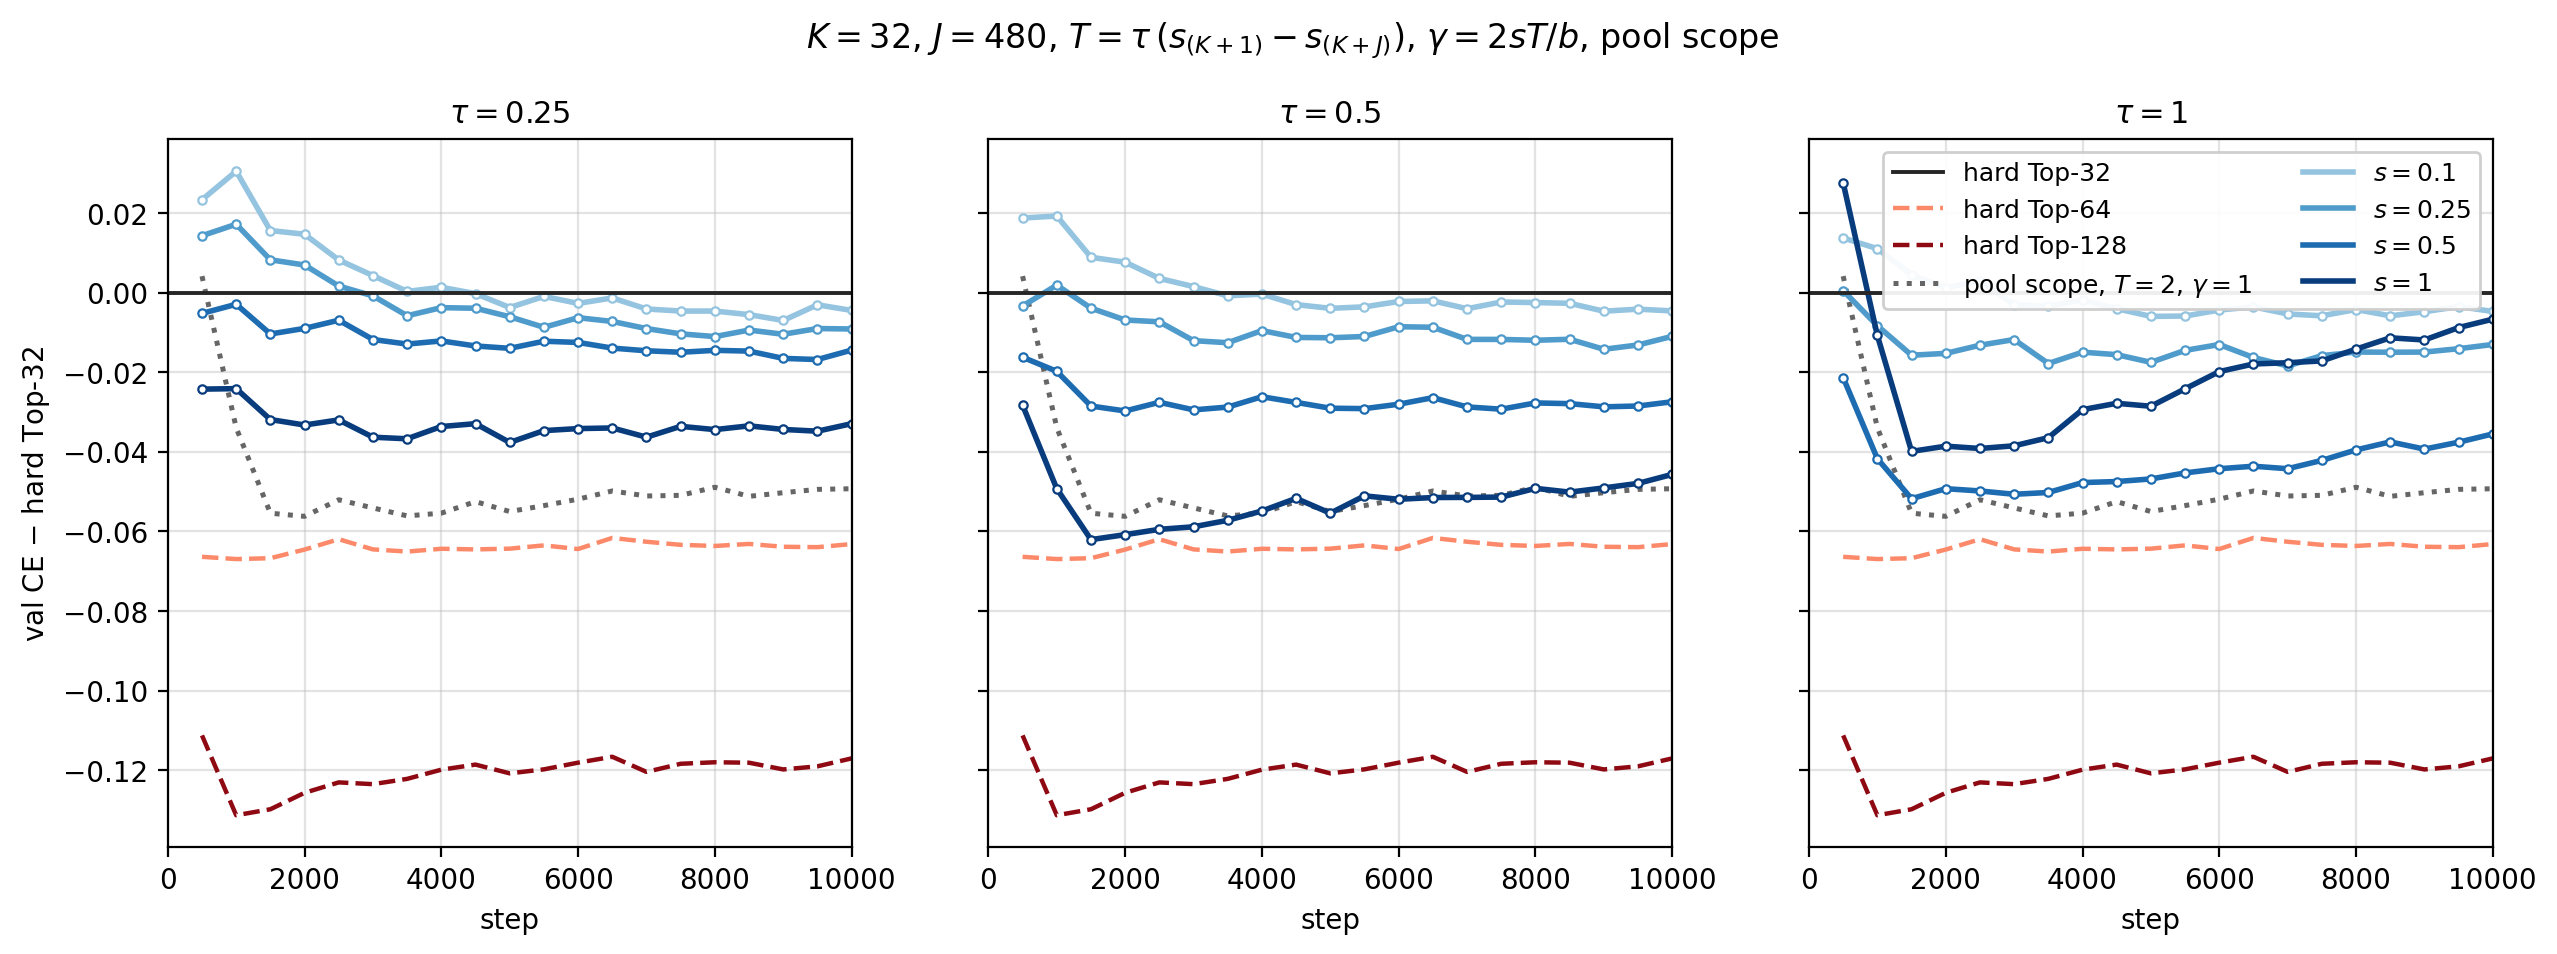
\includegraphics[width=\textwidth]{figures/tsweep/fig_ts_pool_span_k32.png}
\caption{$K = 32$, $J = 480$, span rule, pool scope: validation CE minus
code-carried hard Top-32, one panel per $\tau$, the four strengths as a blue
ramp light to dark with $s$. Dashed: hard Top-64 and Top-128 (reds); dotted
grey: the $T = 2$, $\gamma = 1$ pool-scope run. The ordering in $s$ holds in
every panel; at $\tau = 1$ the $s = 1$ curve is the runaway cell, which leads
until step 3000 and then climbs back towards hard Top-32 as its score scale
grows.}
\label{fig:span32}
\end{figure}

\begin{figure}[htb]\centering
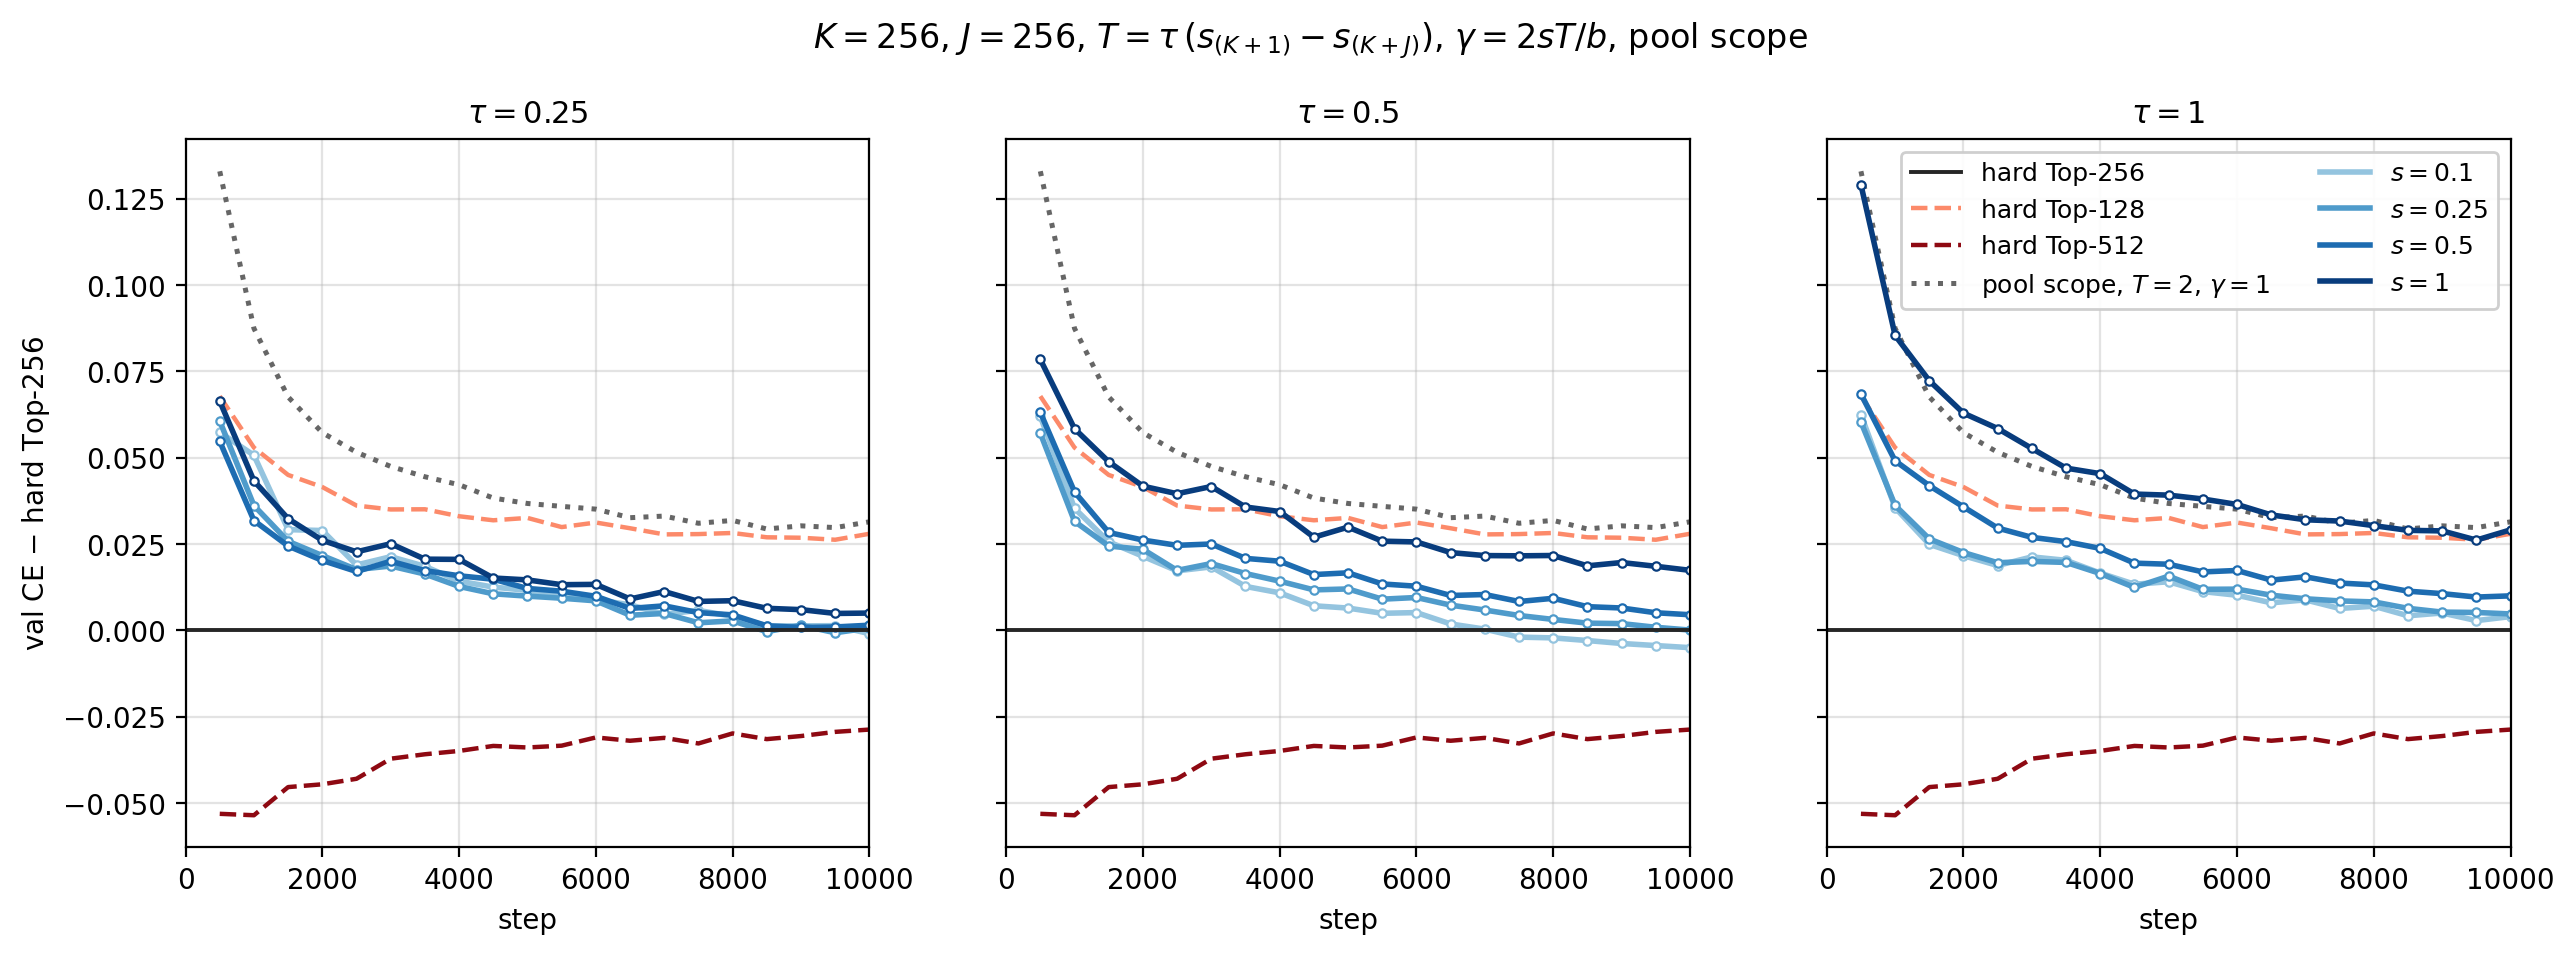
\includegraphics[width=\textwidth]{figures/tsweep/fig_ts_pool_span_k256.png}
\caption{$K = 256$, $J = 256$, span rule, pool scope; same conventions,
with hard Top-128 and hard Top-512 as the dashed references. The curves order
by $s$ in every panel, weakest lowest, and the whole family moves up with
$\tau$; only the $(\tau, s) = (0.5, 0.1)$ curve crosses below hard Top-256,
from step 7000 on. Every curve lies below the dotted $T = 2$, $\gamma = 1$
run from the first validation point except $(1, 1)$, which runs along it.}
\label{fig:span256}
\end{figure}

\begin{figure}[htb]\centering
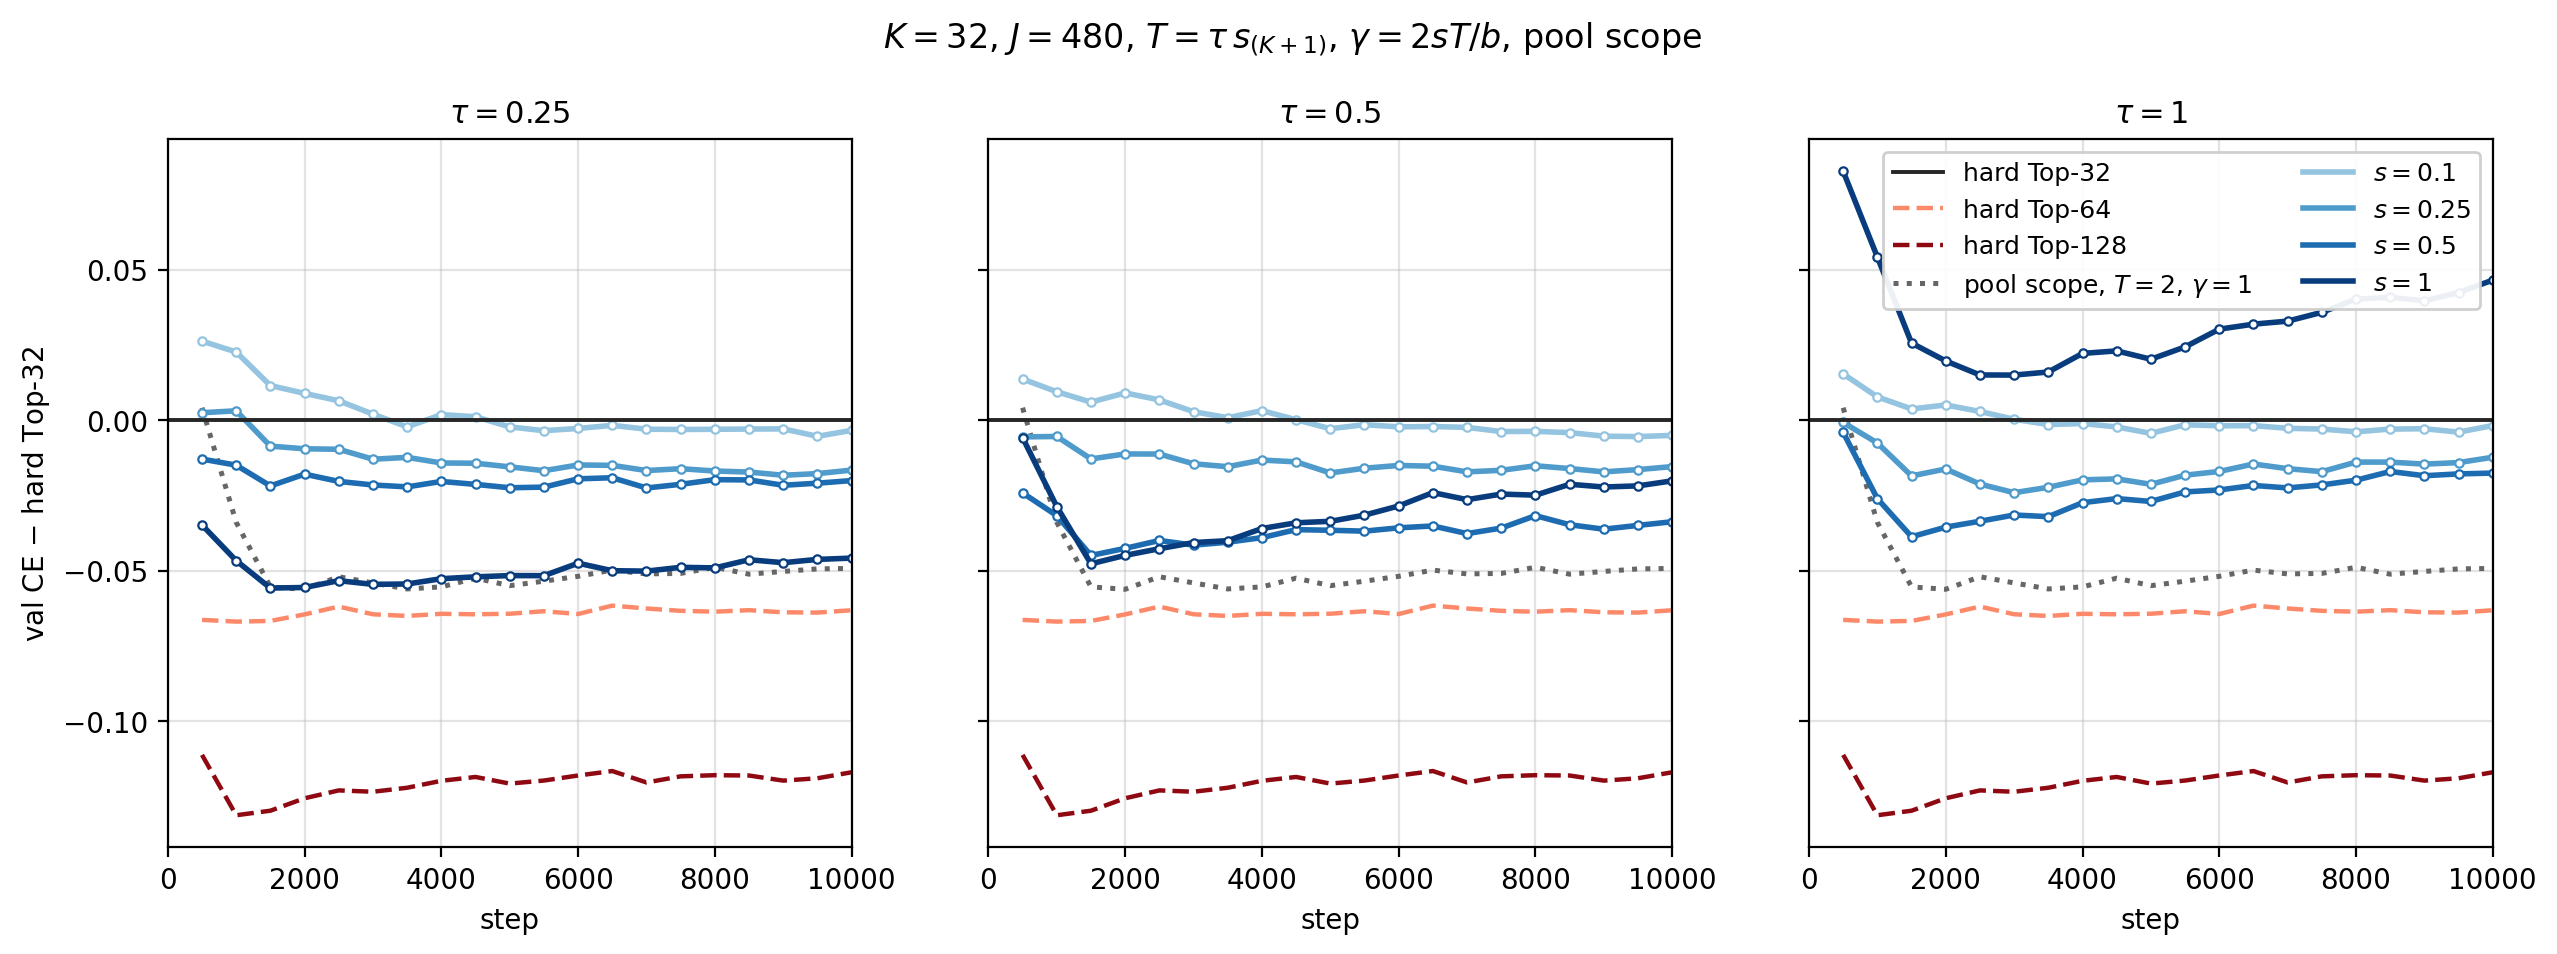
\includegraphics[width=\textwidth]{figures/tsweep/fig_ts_pool_b_k32.png}
\caption{$K = 32$, $J = 480$, $b$ rule, pool scope ($\gamma = 2 s \tau$ in
every cell). The $(\tau, s) = (0.25, 1)$ curve coincides with the $T = 2$,
$\gamma = 1$ run from step 1500 on; the three runaway cells, $(0.5, 1)$,
$(1, 0.5)$ and $(1, 1)$, all with $\gamma \ge 1$, turn upwards after their
early lead, the last one crossing above hard Top-32 at step 4000 and ending
$0.047$ above it.}
\label{fig:b32}
\end{figure}

\begin{figure}[htb]\centering
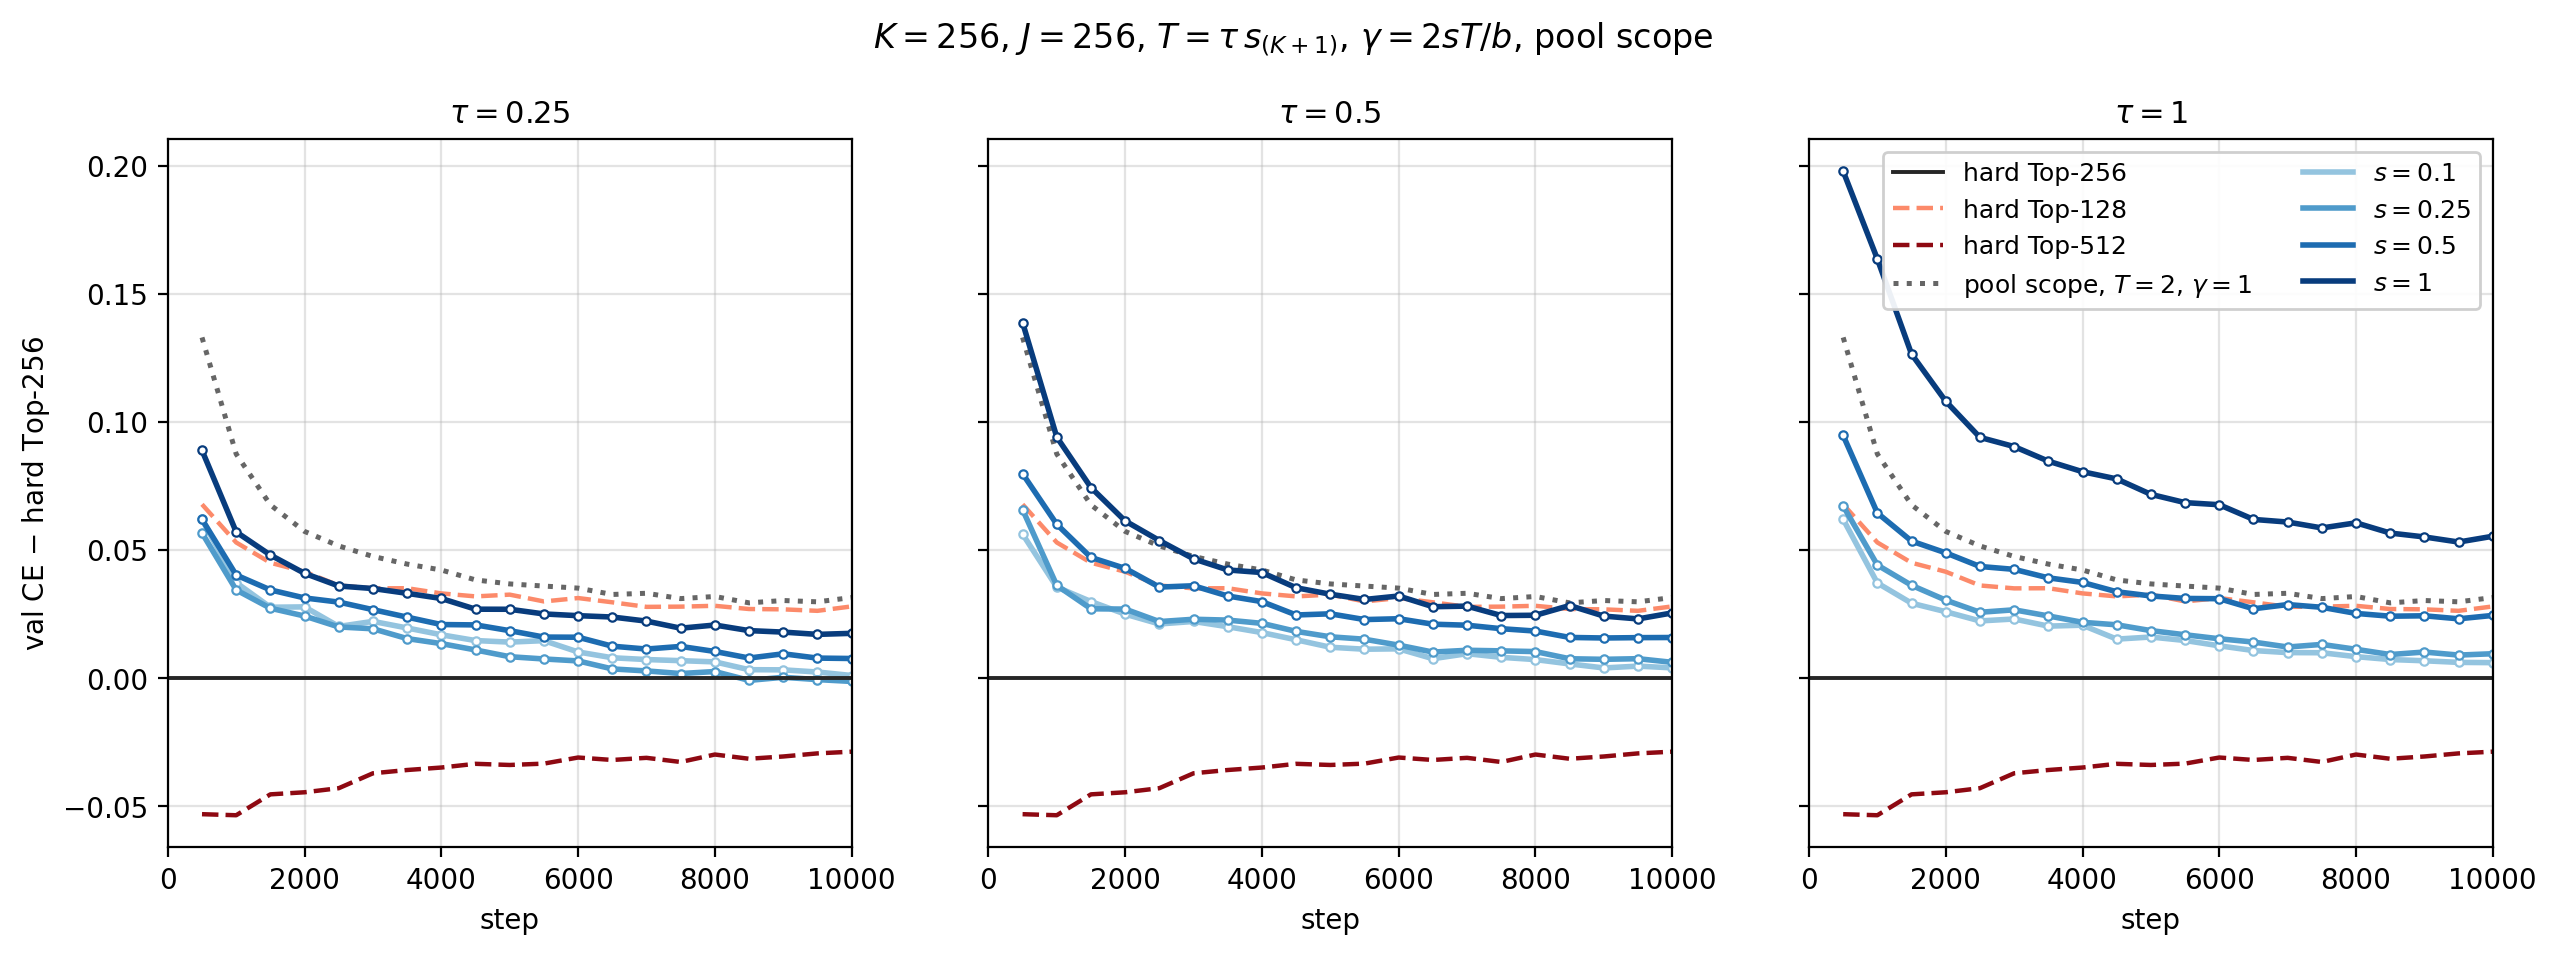
\includegraphics[width=\textwidth]{figures/tsweep/fig_ts_pool_b_k256.png}
\caption{$K = 256$, $J = 256$, $b$ rule, pool scope. Monotone in $s$ and in
$\tau$ throughout; the $(0.25, 0.25)$ curve ends on hard Top-256 and the
$(1, 1)$ curve, $\gamma = 2$, ends $0.055$ above it, the worst cell of the
grid.}
\label{fig:b256}
\end{figure}

\begin{figure}[htb]\centering
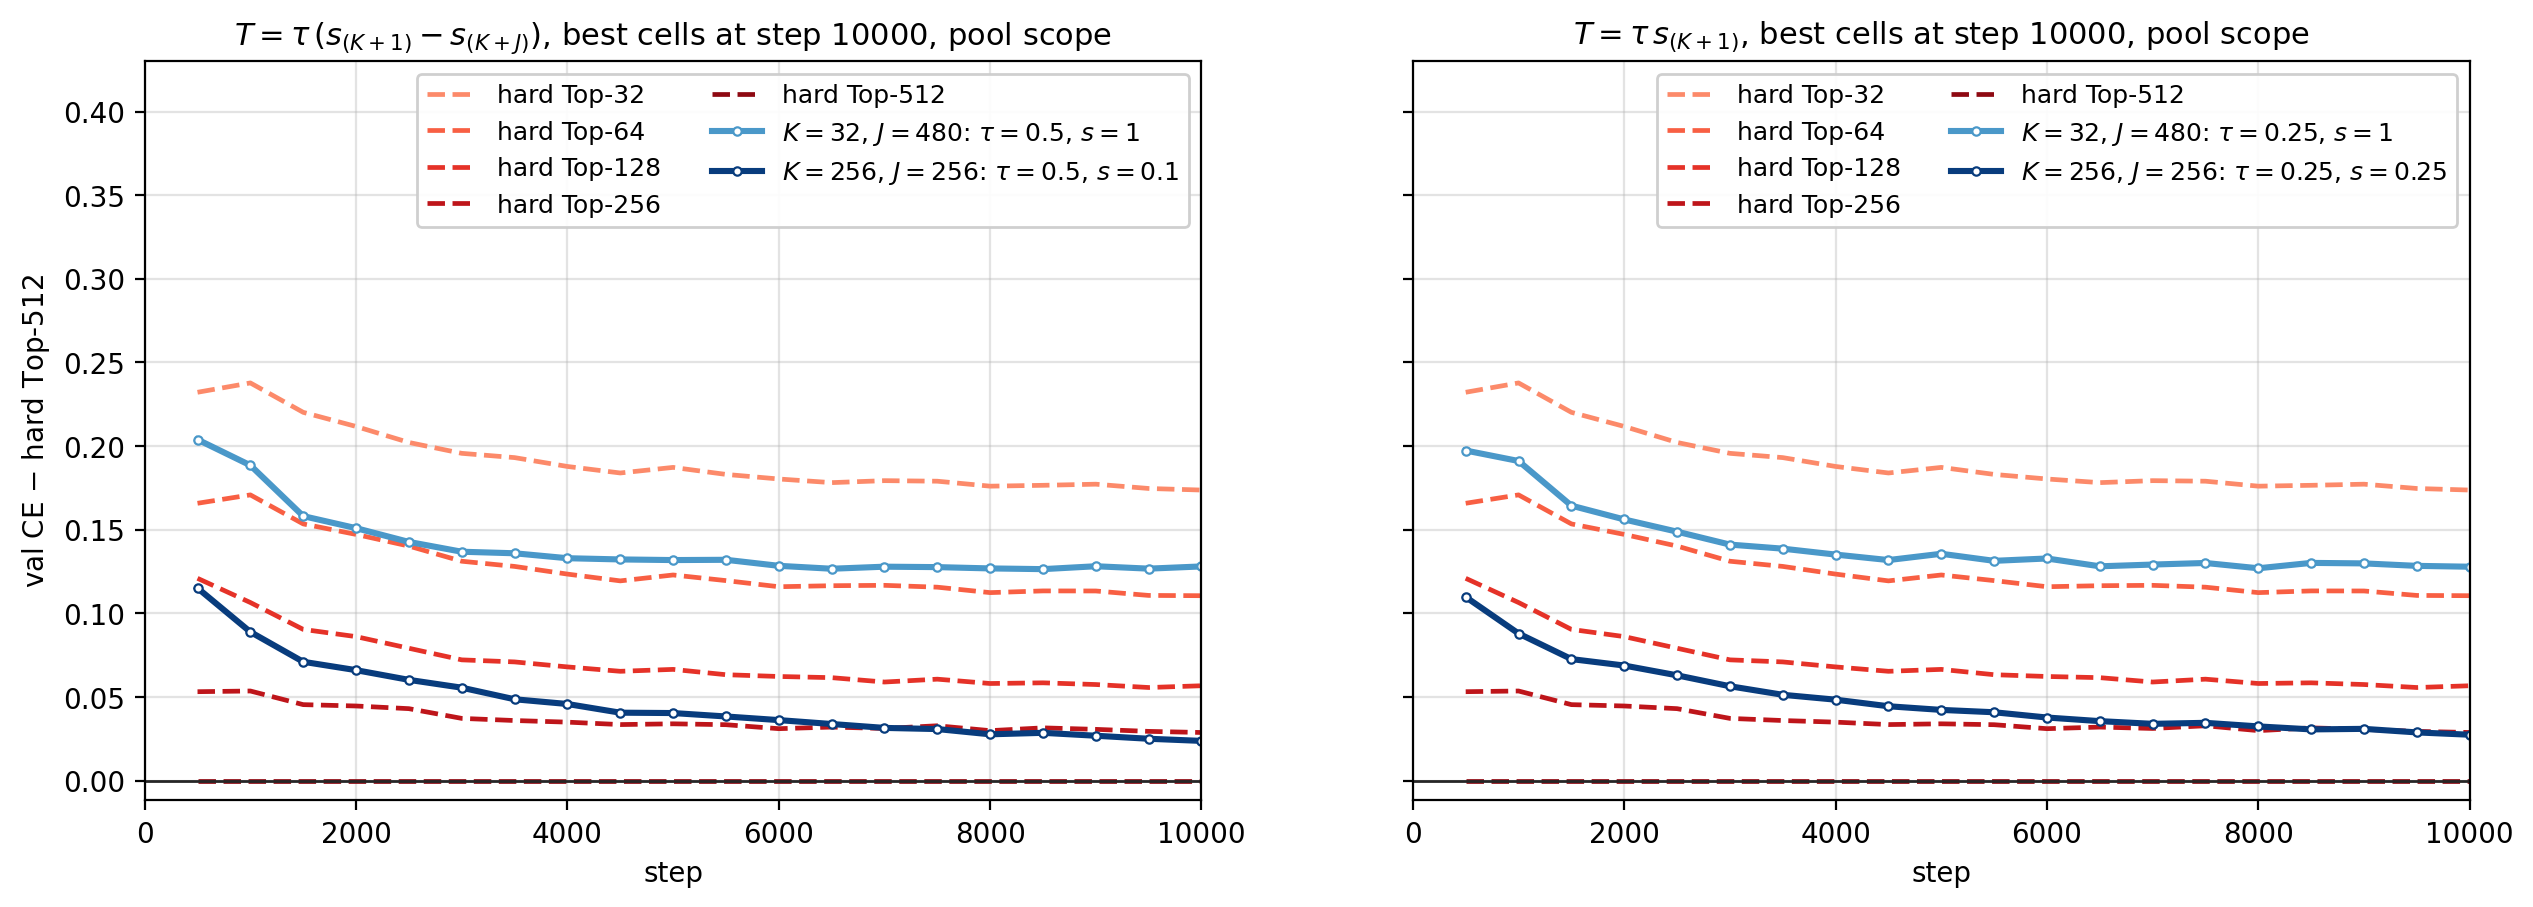
\includegraphics[width=\textwidth]{figures/tsweep/fig_ts_pool_best.png}
\caption{The best cell of each $K$ at step 10000 against the code-carried
hard ladder, validation CE minus hard Top-512; left the span rule, right the
$b$ rule. Dashed: hard Top-$\Kp$ (reds light to dark with $\Kp$); solid: the
best $K = 32$ cell (light blue) and the best $K = 256$ cell (dark blue). Both
$K = 32$ cells end $0.017$ above hard Top-64; both $K = 256$ cells end on
hard Top-256, the span cell $0.005$ below it.}
\label{fig:best}
\end{figure}

% ============================================================
\subsection{The score scale}
\label{sec:stab}
% ============================================================

No run diverged in the sense of the guard (training CE more than $2.5$ above
its best for 800 steps), and the gradient norms stayed between $0.2$ and
$0.4$ in every run. Four cells nevertheless left the regime of the others: the
boundary score $b$, which falls slowly from about $2.6$ at step 1000 to
$0.8$--$1.5$ at step 10000 in the weak cells, grows in them instead, and the
cell's loss advantage decays as it grows. The boundary score at step 10000,
averaged over tokens and blocks:

\begin{center}\small
\begin{tabular}{l|cccc|cccc}
\toprule
$b$ at step 10000 & \multicolumn{4}{c|}{span rule, $K = 32$} & \multicolumn{4}{c}{$b$ rule, $K = 32$} \\
$\tau$ & $s{=}0.1$ & $0.25$ & $0.5$ & $1$ & $s{=}0.1$ & $0.25$ & $0.5$ & $1$ \\
\midrule
$0.25$ & 1.44 & 1.22 & 1.00 & 0.82 & 1.33 & 1.11 & 0.98 & 1.36 \\
$0.5$  & 1.28 & 1.08 & 1.18 & 3.47 & 1.25 & 1.24 & 2.23 & 29.9 \\
$1$    & 1.27 & 1.49 & 3.94 & 180 & 1.44 & 2.45 & 12.5 & 1561 \\
\midrule
& \multicolumn{4}{c|}{span rule, $K = 256$} & \multicolumn{4}{c}{$b$ rule, $K = 256$} \\
\midrule
$0.25$ & 1.16 & 1.11 & 1.11 & 1.01 & 1.05 & 0.93 & 0.76 & 0.63 \\
$0.5$  & 1.11 & 1.00 & 0.85 & 0.72 & 0.92 & 0.74 & 0.63 & 1.62 \\
$1$    & 0.94 & 0.76 & 0.64 & 0.66 & 0.93 & 0.92 & 1.38 & 3.43 \\
\bottomrule
\end{tabular}
\end{center}

At $K = 32$ the cells with a realized $\gamma \ge 1$ -- span $(1, 1)$ with
$\gamma = 1.1$, $b$-rule $(0.5, 1)$ and $(1, 0.5)$ with $\gamma = 1$, and
$(1, 1)$ with $\gamma = 2$ -- reach $b = 12$ to $1561$; the cells at $\gamma
= 0.5$--$0.6$ sit at $2.2$--$3.9$, two to three times the weak cells; below
that $b$ is $0.8$--$1.5$ as in the hard runs. In the span cell $(1, 1)$ the
growth is exponential from step 3000 on:

\begin{center}\footnotesize
\begin{tabular}{lccccccccc}
\toprule
step & 1000 & 2000 & 3000 & 4000 & 5000 & 6000 & 7000 & 8000 & 10000 \\
\midrule
$b$ & 6.1 & 7.9 & 10.6 & 14.2 & 20.8 & 31.6 & 51.4 & 81.0 & 180.3 \\
$\Delta$ to hard Top-32 & $-0.011$ & $-0.039$ & $-0.039$ & $-0.029$ & $-0.029$ & $-0.020$ & $-0.018$ & $-0.014$ & $-0.007$ \\
\bottomrule
\end{tabular}
\end{center}

a factor $1.5$--$1.6$ per thousand steps, while the realized $\gamma$ stays
at $1.1$--$1.2$ and the realized $T$ grows with $b$ (to $121$). The cell led
hard Top-32 by $0.039$ at steps 2000--3000, as much as the best cells, and
gave up five sixths of it by step 10000. The $b$-rule cell $(1, 1)$ did the
same faster and ended above hard Top-32. The fixed configuration, $T = 2$,
$\gamma = 1$, keeps $b$ near $2.3$ to the end of a 20k run.

At $K = 256$ the strong cells move the other way: $b$ falls to $0.63$--$0.66$
at $(\tau, s) = (1, 1)$ under the span rule and at $(0.25, 1)$, $(0.5, 0.5)$
under the $b$ rule, against $1.0$--$1.2$ in the weak cells; only the two
$b$-rule cells with $\gamma \ge 1$ grow, to $1.6$ and $3.4$.

% ============================================================
\section{Interpretation}
% ============================================================

Three readings follow from the measurements; the first two are supported by
the grid, the third is a hypothesis.

First, \textbf{the grid recovers the fixed configuration but does not
improve on it at $K = 32$.} The best cells of both rules end within $0.004$ of
the $T = 2$, $\gamma = 1$ run and have a realized scale of $0.5$--$0.6$, where
that run's realized strength $s = b/4$ is $0.2$--$0.5$ over most of training
with a width covering the pool. The loss falls monotonically towards the
strong-and-wide corner and stops where the score scale becomes unstable, so
the fixed configuration already sits near the optimum of this family, and
what limits the code-carried surrogate at $K = 32$ is not the choice of
reach or strength.

Second, \textbf{the relative rules remove the anchor of the score scale.}
With $T \propto b$ (or $\propto$ span, which tracks $b$) and $\gamma \propto
T/b$ the support term \eqref{eq:support} is unchanged by a common rescaling
of the scores, and the four cells with $\gamma \ge 1$ show that the gradient
then drives the scale upwards without bound. At fixed $T$ a growing $b$
narrows the kernel relative to the pool and increases $\kappa$ at the
boundary only as $1/2T$, which is what keeps the $T = 2$ run at $b \approx
2.3$. A relative rule that is to be used at $\gamma \ge 1$ would need an
explicit anchor, for instance a fixed $T$ for the kernel together with a
relative $\gamma$, or a penalty on $b$; the grid did not test one.

Third, the \textbf{$K$-dependence}. At $K = 32$ more strength and more reach
help; at $K = 256$ both hurt and the best cells are near zero. The hard
ladder gives the scale of what a better support can be worth: the gain per
added feature at the margin is $2.0 \times 10^{-3}$ between Top-32 and Top-64
and $1.1 \times 10^{-4}$ between Top-256 and Top-512, an 18-fold drop, while
the costs of the term -- the bias it puts on the gradient of the active
features and its action along the carry -- are set by $s$ and $\tau$ and do
not shrink with $K$. The direction matches; the size does not entirely: the
$T = 2$ run recovers $0.049$ of the $0.063$ doubling gain at $K = 32$, and the
same fraction of the $0.029$ gain at $K = 256$ would be $0.023$, where the
best cells recover $0.005$. The remainder is what the carry studies
attributed to the term's action along the carried code, which the pool
scope keeps in every cell here.

% ============================================================
\section{Scope}
% ============================================================

All cells are single runs at one seed, and the comparisons are at step
10000 of a 20k schedule, not at convergence; in the earlier studies the
ranking of methods moved by up to a quarter of the gaps between 3k and 10k
steps. Differences below about $0.005$ are within what one config produces
on two machines. The hard baselines carry the output norm and the surrogate
cells do not, as in the K+J notes, except for the eight post-norm cells of
Section~\ref{sec:fo-pnorm}. The grid changes the kernel width and the
scale and keeps everything else of the code-carried $T = 2$ cell, including
the pool scope, so the term's action along the carry is present in every
cell. Only two $(K, J)$ cells were run, both at $K + J = 512$.

% ============================================================
\section{The first-order arm}
\label{sec:fo}
% ============================================================

The span rule of the grid, $\tau \in \{0.25, 0.5, 1\}$, $s \in \{0.1, 0.25,
0.5, 1\}$, at $(32, 480)$ and $(256, 256)$, repeated with the scope
\code{rblapsum\_surrogate\_scope} $=$ \code{first\_order}: each gate's support
term is evaluated on the gradient that reached it along hard paths, so no
gradient carries more than one support term and the products of terms along
the carry are removed (\code{docs/kj-vs-hard-topk-code-residual.tex},
Section~6). The kernel width and the strength are set per token exactly as in
the pool arm, and the realized $\gamma$ at step 10000 agrees with the pool
arm's cell by cell to within $0.01$. The reference of this arm is the
first-order $T = 2$, $\gamma = 1$ cell of the K+J grid,
\code{ma\_cr\_rbk\_k<K>\_j<J>\_t2\_fo}, at $1.6322$ ($-0.024$ against hard
Top-32) and $1.5285$ ($+0.018$ against hard Top-256) at step 10000. The 24
runs (\code{ma\_ts\_span\_*\_fo}) train at $0.60$ s per step, against $0.41$
for the pool scope, because the first-order backward is a second backward
pass. None diverged.

Validation CE at step 10000 minus hard Top-$K$; in parentheses the
pool-scope cell with the same $(\tau, s)$ from Section~4. Bold marks the best
cell of the arm, a dagger a score-scale runaway.

\begin{center}\small
\begin{tabular}{l|cccc}
\toprule
$K = 32$, $J = 480$, $\tau$ & $s{=}0.1$ & $0.25$ & $0.5$ & $1$ \\
\midrule
$0.25$ & $-0.004$ ($-0.005$) & $-0.012$ ($-0.009$) & $-0.018$ ($-0.014$) & $\mathbf{-0.028}$ ($-0.033$) \\
$0.5$  & $-0.005$ ($-0.005$) & $-0.009$ ($-0.011$) & $-0.020$ ($-0.027$) & $-0.024$ ($-0.046$) \\
$1$    & $-0.006$ ($-0.005$) & $-0.011$ ($-0.013$) & $-0.011$ ($-0.036$) & $+0.034^\dagger$ ($-0.007^\dagger$) \\
\midrule
first-order $T{=}2$, $\gamma{=}1$ & \multicolumn{4}{c}{$-0.024$ \quad (pool scope: $-0.049$)} \\
\bottomrule
\end{tabular}
\end{center}

\begin{center}\small
\begin{tabular}{l|cccc}
\toprule
$K = 256$, $J = 256$, $\tau$ & $s{=}0.1$ & $0.25$ & $0.5$ & $1$ \\
\midrule
$0.25$ & $+0.005$ ($-0.001$) & $0.000$ ($+0.001$) & $+0.001$ ($+0.002$) & $+0.002$ ($+0.005$) \\
$0.5$  & $+0.001$ ($-0.005$) & $\mathbf{0.000}$ ($0.000$) & $+0.001$ ($+0.005$) & $+0.008$ ($+0.017$) \\
$1$    & $+0.001$ ($+0.004$) & $+0.001$ ($+0.005$) & $+0.006$ ($+0.010$) & $+0.017$ ($+0.029$) \\
\midrule
first-order $T{=}2$, $\gamma{=}1$ & \multicolumn{4}{c}{$+0.018$ \quad (pool scope: $+0.031$)} \\
\bottomrule
\end{tabular}
\end{center}

\paragraph{$K = 32$.}
At the narrowest width the two scopes agree to within $0.005$ at every $s$,
the first-order scope ahead at $s = 0.25$ and $0.5$ and behind at $s = 1$.
Widening the kernel separates them: at $\tau = 0.5$ the first-order cells
trail the pool cells by $0.007$ and $0.022$ at $s = 0.5$ and $1$, at $\tau =
1$ by $0.025$ at $s = 0.5$, and the first-order loss no longer improves with
$\tau$ at any $s \ge 0.25$. Its best cell, $(\tau, s) = (0.25, 1)$ at
$-0.028$, is $0.004$ better than the first-order $T = 2$, $\gamma = 1$ run and
$0.018$ behind the pool scope's best cell. The pool scope's extra gain at wide
kernels is therefore carried by the products of support terms along the
carry, which the first-order scope removes: the K+J note measured this at
$T = 2$ as a cost of $0.007$--$0.024$ for the first-order scope at $K = 32$,
and the grid finds the same sign and size at every width that reaches the
whole pool.

\paragraph{The score scale.}
The runaway of Section~\ref{sec:stab} does not depend on the products along
the carry. The first-order cell $(1, 1)$ at $K = 32$, realized $\gamma =
1.3$, grows its boundary score from $6.0$ at step 1000 to $12$, $41$, $103$
and $224$ at steps 3000, 6000, 8000 and 10000, the same factor of $1.5$--$1.6$
per thousand steps as the pool cell, and ends $0.034$ above hard Top-32 after
a lead of $0.007$ at step 2000; the two cells at $\gamma \approx 0.65$,
$(0.5, 1)$ and $(1, 0.5)$, sit at $b = 4.2$ and $4.7$, as the pool cells at
that scale do. At $K = 256$ the boundary score falls with $\tau s$ as in the
pool arm, to $0.51$ at $(1, 1)$.

\paragraph{$K = 256$.}
The first-order scope flattens the table: at $s \le 0.5$ every cell is within
$0.006$ of hard Top-256, and the strong cells lose about half of what the
pool cells lose ($+0.008$ against $+0.017$ at $(0.5, 1)$, $+0.017$ against
$+0.029$ at $(1, 1)$). No cell is below hard Top-256 by more than $0.0002$,
and the weak-and-moderate corner, where the pool scope found its $-0.005$, is
at $+0.001$ to $+0.005$ here. All 24 cells beat the first-order $T = 2$,
$\gamma = 1$ run.

\begin{figure}[htb]\centering
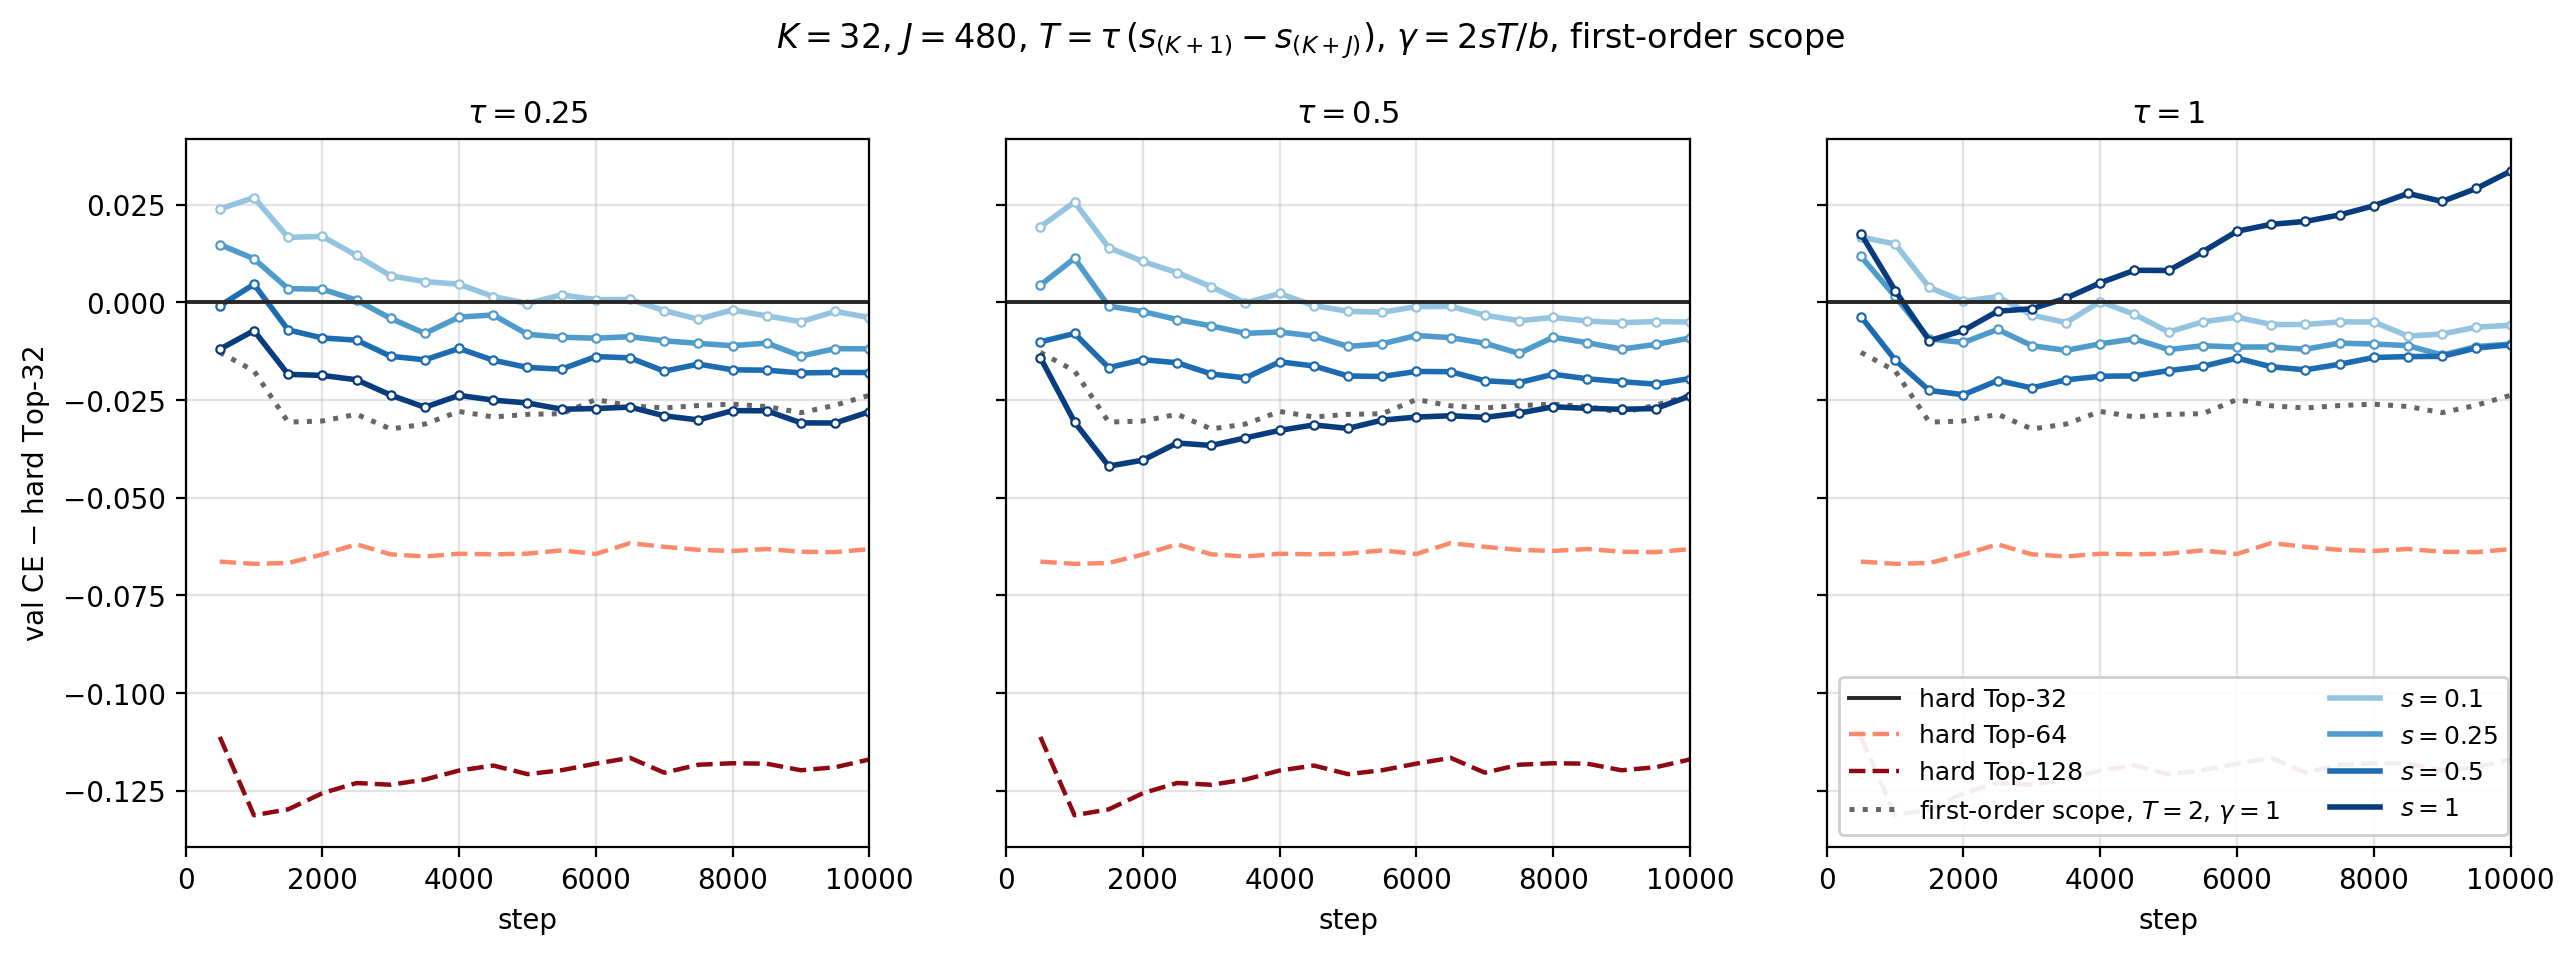
\includegraphics[width=\textwidth]{figures/tsweep/fig_ts_fo_span_k32.png}
\caption{$K = 32$, $J = 480$, span rule, first-order scope; conventions as in
Figure~\ref{fig:span32}, the dotted grey curve now the first-order $T = 2$,
$\gamma = 1$ run. The $s = 1$ curve is the lowest only at $\tau = 0.25$; at
$\tau = 0.5$ it meets the $s = 0.5$ curve from step 5000 on, and at $\tau = 1$
it is the runaway cell, which crosses above hard Top-32 at step 3500 and ends
$0.034$ above it.}
\label{fig:fo32}
\end{figure}

\begin{figure}[htb]\centering
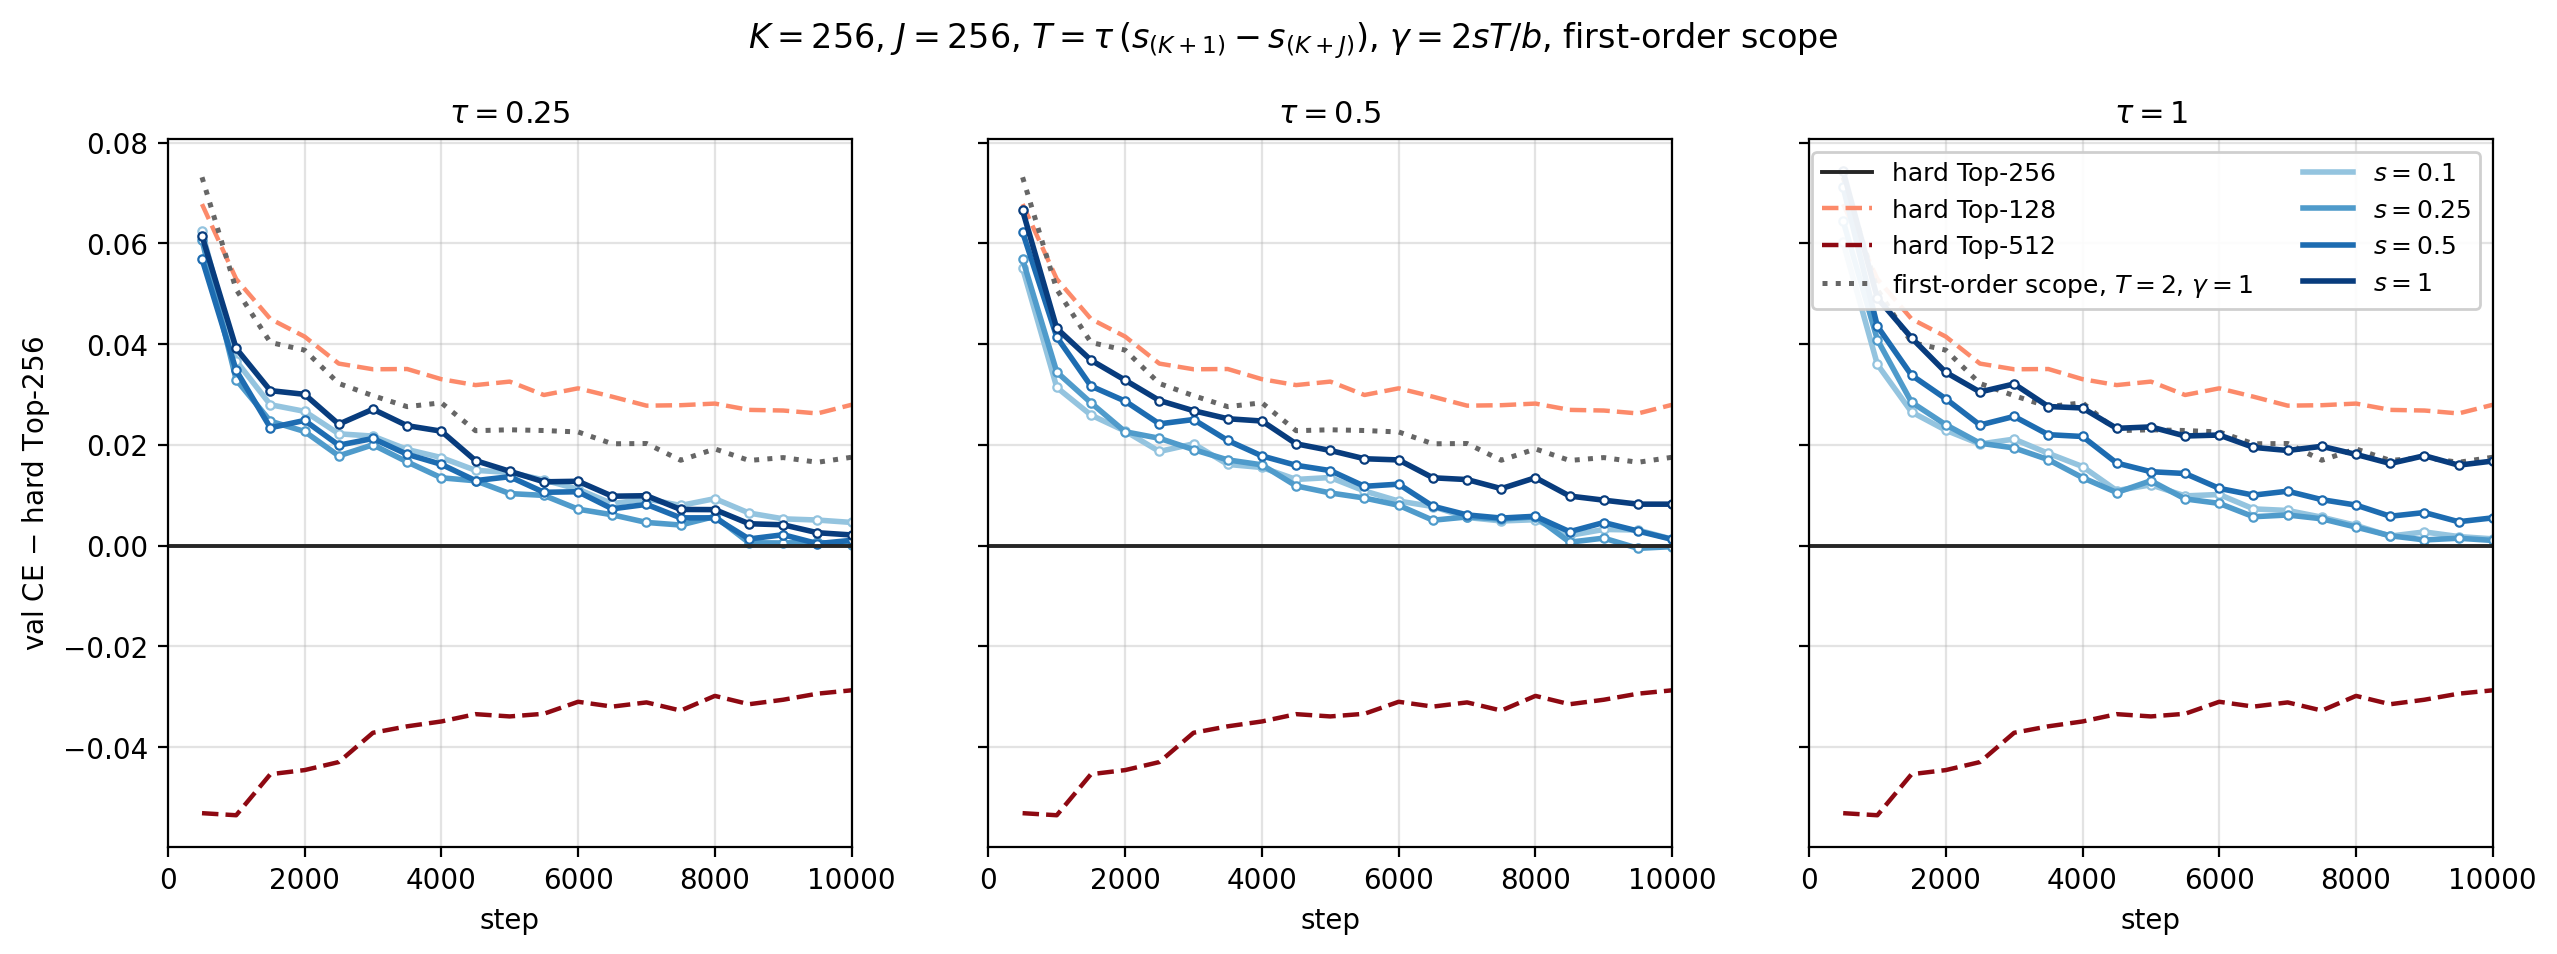
\includegraphics[width=\textwidth]{figures/tsweep/fig_ts_fo_span_k256.png}
\caption{$K = 256$, $J = 256$, span rule, first-order scope. The $s \le 0.5$
curves of all three panels converge onto hard Top-256 from step 7000 on; only
the $s = 1$ curves stay above, by less than the pool-scope cells of
Figure~\ref{fig:span256}.}
\label{fig:fo256}
\end{figure}

\begin{figure}[htb]\centering
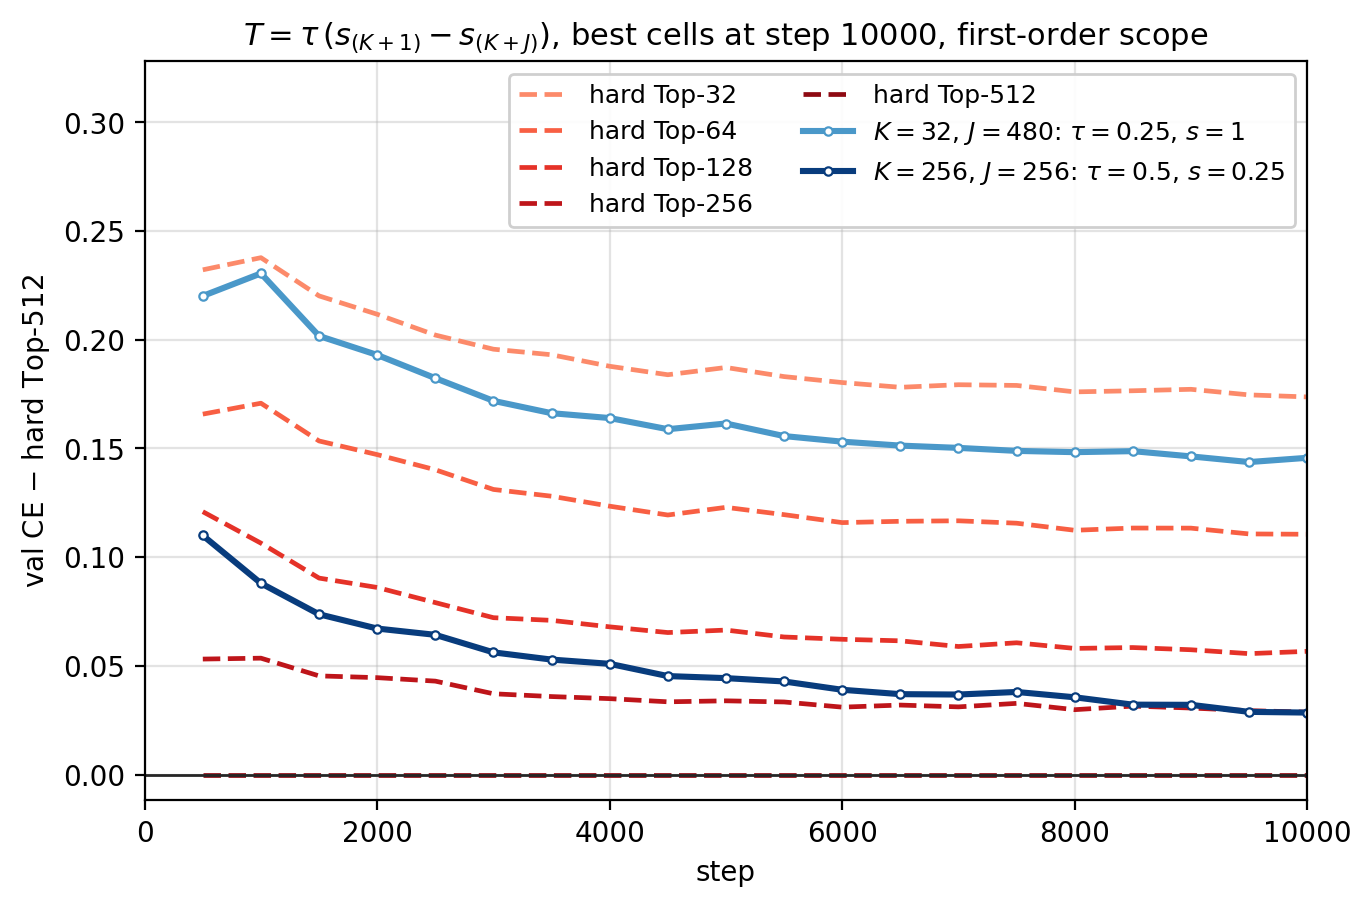
\includegraphics[width=.6\textwidth]{figures/tsweep/fig_ts_fo_best.png}
\caption{The best first-order cell of each $K$ at step 10000 against the
code-carried hard ladder, as in Figure~\ref{fig:best}. The $K = 32$ cell,
$(0.25, 1)$, ends $0.035$ above hard Top-64 (the pool scope's best:
$0.017$); the $K = 256$ cell, $(0.5, 0.25)$, ends on hard Top-256.}
\label{fig:fobest}
\end{figure}

% ============================================================
\subsection{The output norm}
\label{sec:fo-pnorm}
% ============================================================

Every surrogate cell of this note is trained without the RMSNorm on the
bottleneck's decoded output, while the hard baselines carry it. To see what
the norm does to the first-order cells, two columns of the span grid were
repeated with \code{post\_norm} $=$ \code{true} and nothing else changed:
$(K, J) = (32, 480)$ at $\tau = 0.5$ and $(256, 256)$ at $\tau = 0.25$, the
four strengths each, eight runs
(\code{configs/cr\_kj/tsweep/de\_ts\_span\_*\_fo\_pnorm.yaml}, trained on
denver, 10k steps of the 20k schedule as above; \code{scripts/plot\_tsweep\_pnorm.py}).
Validation CE at step 10000 minus hard Top-$K$, the cells without the norm
from the tables above in parentheses:

\begin{center}\small
\begin{tabular}{l|cccc}
\toprule
first-order, span rule, post-norm & $s{=}0.1$ & $0.25$ & $0.5$ & $1$ \\
\midrule
$K = 32$, $J = 480$, $\tau = 0.5$ & $-0.005$ ($-0.005$) & $-0.007$ ($-0.009$) & $-0.021$ ($-0.020$) & $-0.017$ ($-0.024$) \\
$K = 256$, $J = 256$, $\tau = 0.25$ & $-0.001$ ($+0.005$) & $0.000$ ($0.000$) & $+0.001$ ($+0.001$) & $-0.002$ ($+0.002$) \\
\bottomrule
\end{tabular}
\end{center}

The end points move by at most $0.007$, and the ordering in $s$ is kept at
$K = 32$ ($s = 0.5$ and $s = 1$ remain the best two cells, now in the other
order). What changes is the course of training
(Figure~\ref{fig:fopnorm}). At $K = 32$ the cells without the norm dip to
$-0.03$ to $-0.04$ at steps 1500--2000 and then give part of it back; with the
norm the same cells start $0.045$ below hard Top-32 at step 500 and approach
their end points monotonically, so the early lead of the strong cells is
gone and so is its decay. At $K = 256$ the cells without the norm start
$0.06$ above hard Top-256 and need until step 8000 to reach it; with the norm
all four are within $\pm 0.004$ of it from step 1000 on, and none is below it
by more than $0.002$ at the end. The norm removes the slow approach of the
surrogate cells to the hard baseline at $K = 256$ without producing a gain
over it, and at $K = 32$ it leaves the margin of the first-order scope at
$0.02$, half the pool scope's.

\begin{figure}[htb]\centering
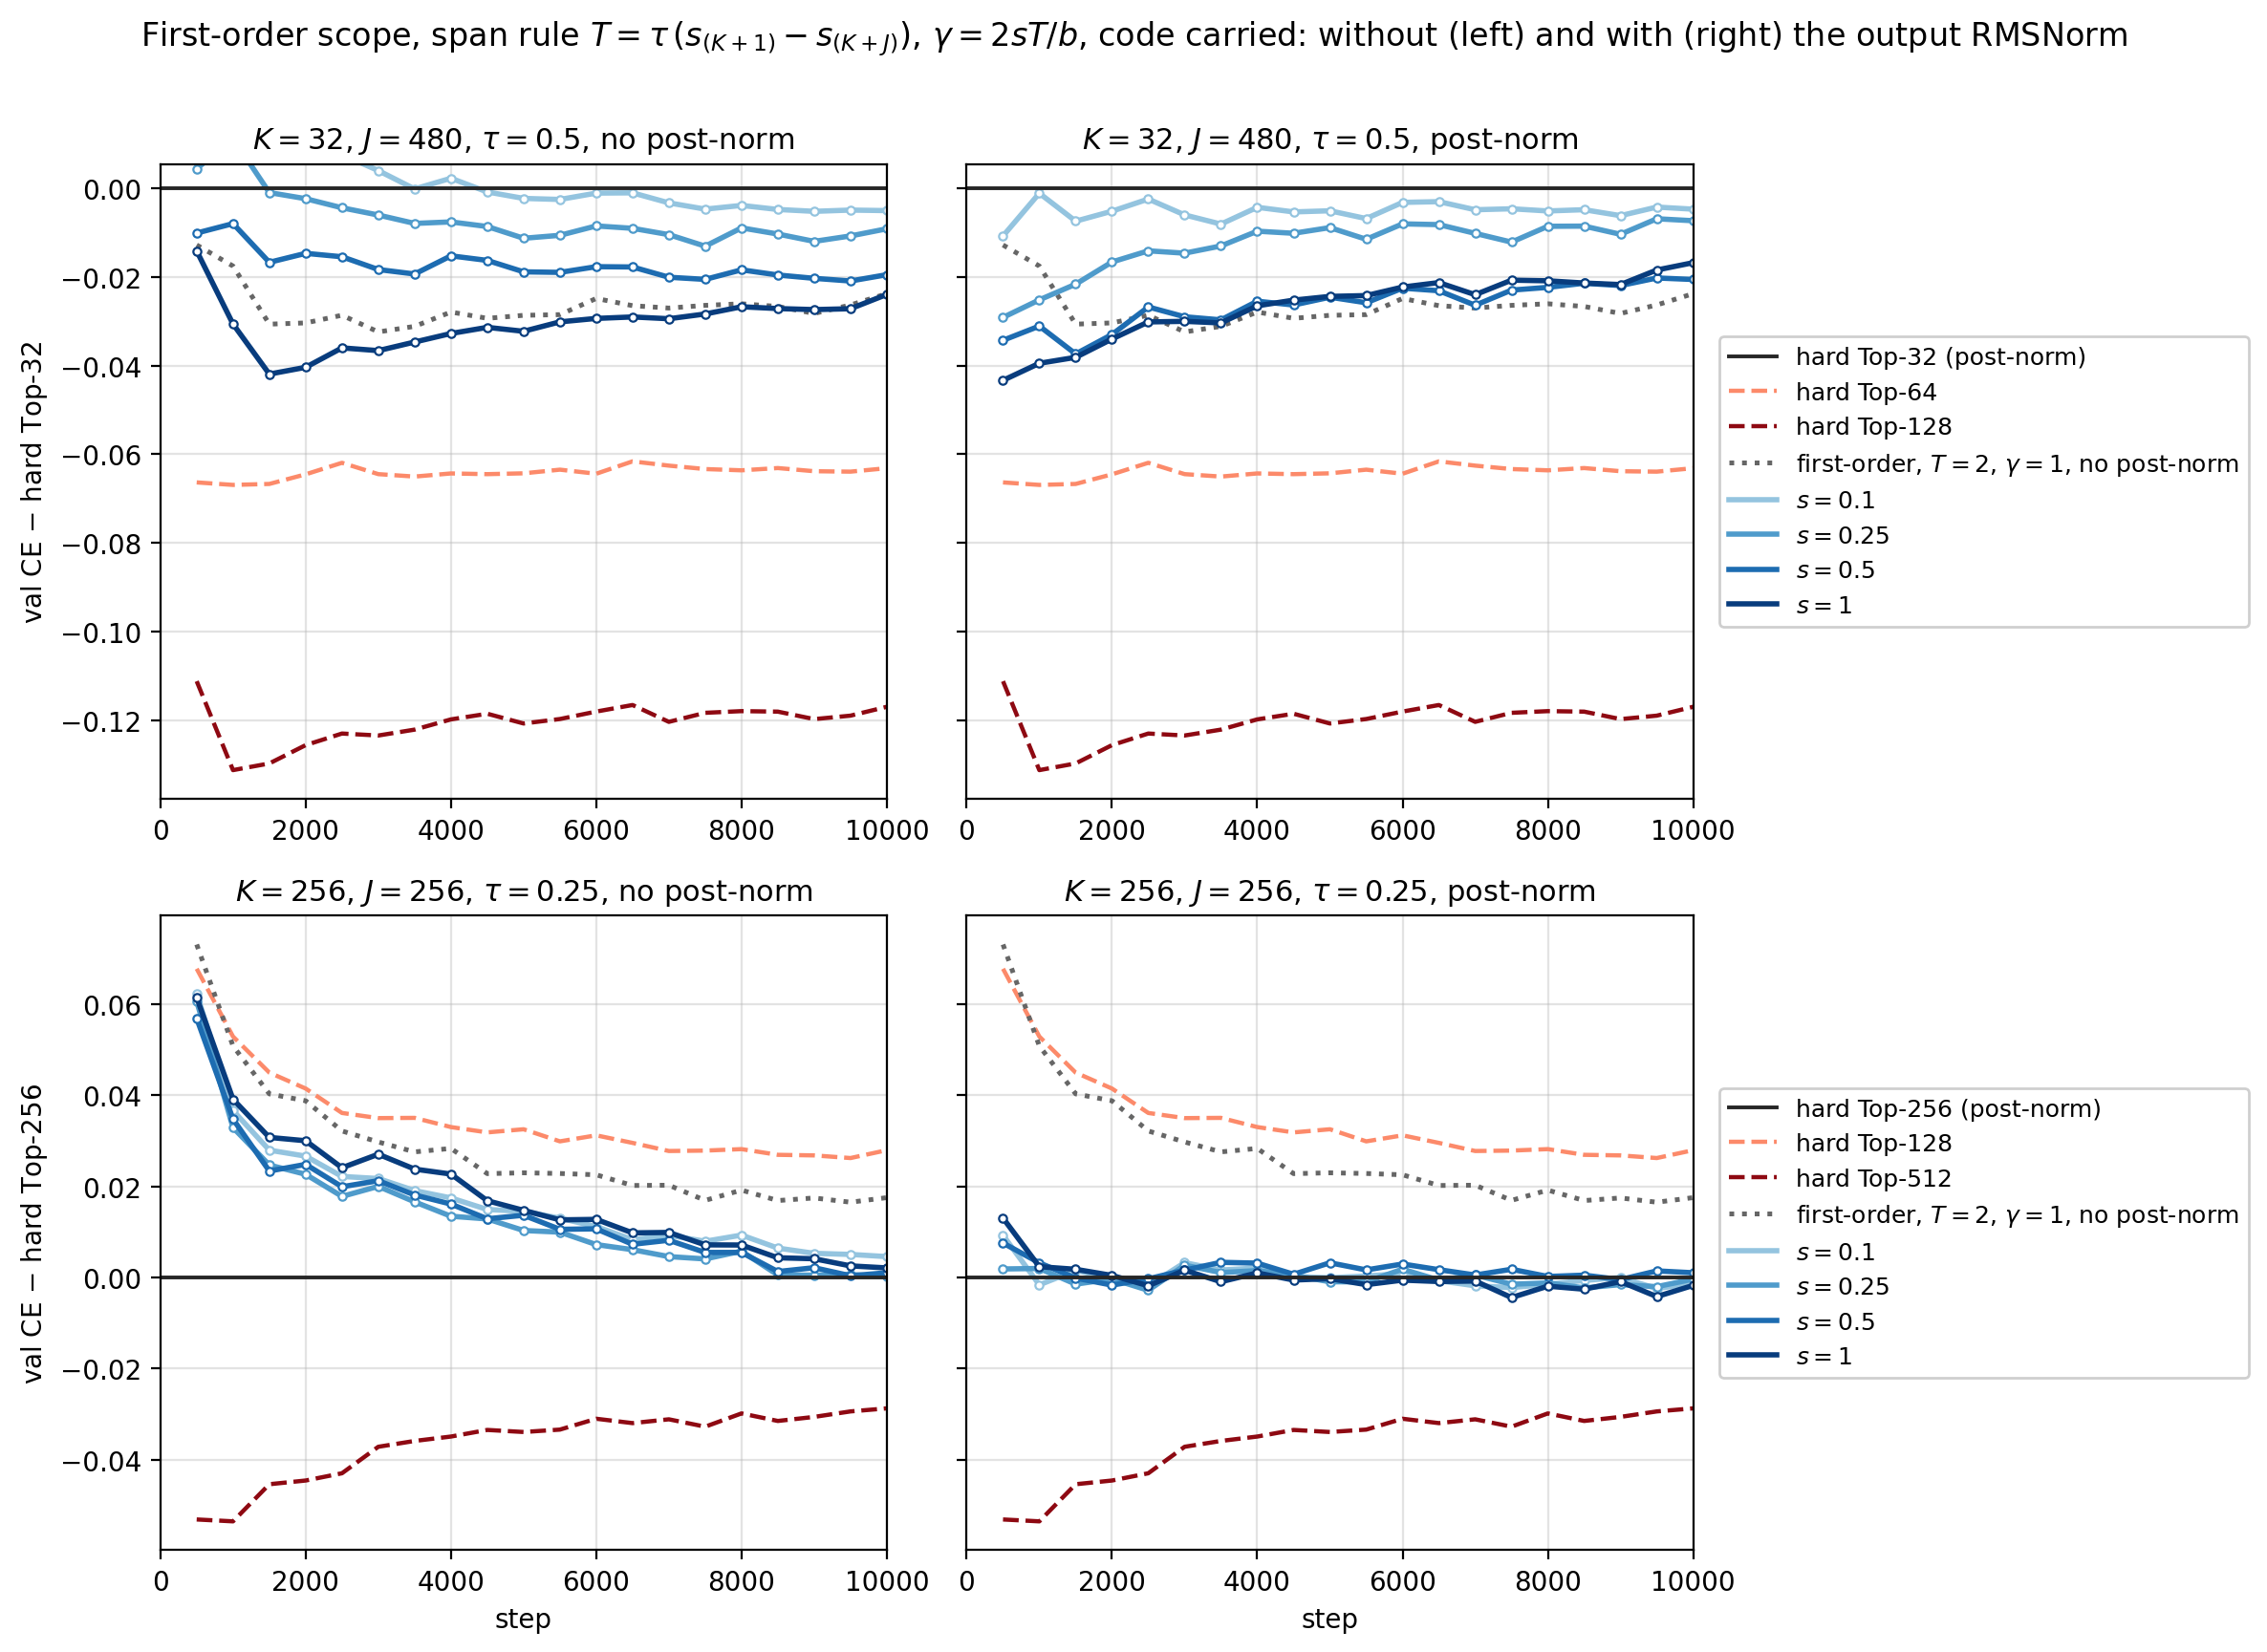
\includegraphics[width=\textwidth]{figures/tsweep/fig_ts_fo_span_pnorm.png}
\caption{First-order scope, span rule, without (left, the middle panel of
Figure~\ref{fig:fo32} and the left panel of Figure~\ref{fig:fo256}) and with
(right) the output RMSNorm; top $K = 32$, $J = 480$, $\tau = 0.5$, bottom
$K = 256$, $J = 256$, $\tau = 0.25$. Conventions as before; the dotted grey
curve is the first-order $T = 2$, $\gamma = 1$ run without the norm in both
columns. With the norm the $K = 32$ cells approach their end points from
below without the dip at steps 1500--2000, and the $K = 256$ cells lie on
hard Top-256 from step 1000 on.}
\label{fig:fopnorm}
\end{figure}

\end{document}
